\documentclass{standalone}
\usepackage{tikz}
\usetikzlibrary{patterns, positioning}


\begin{document}
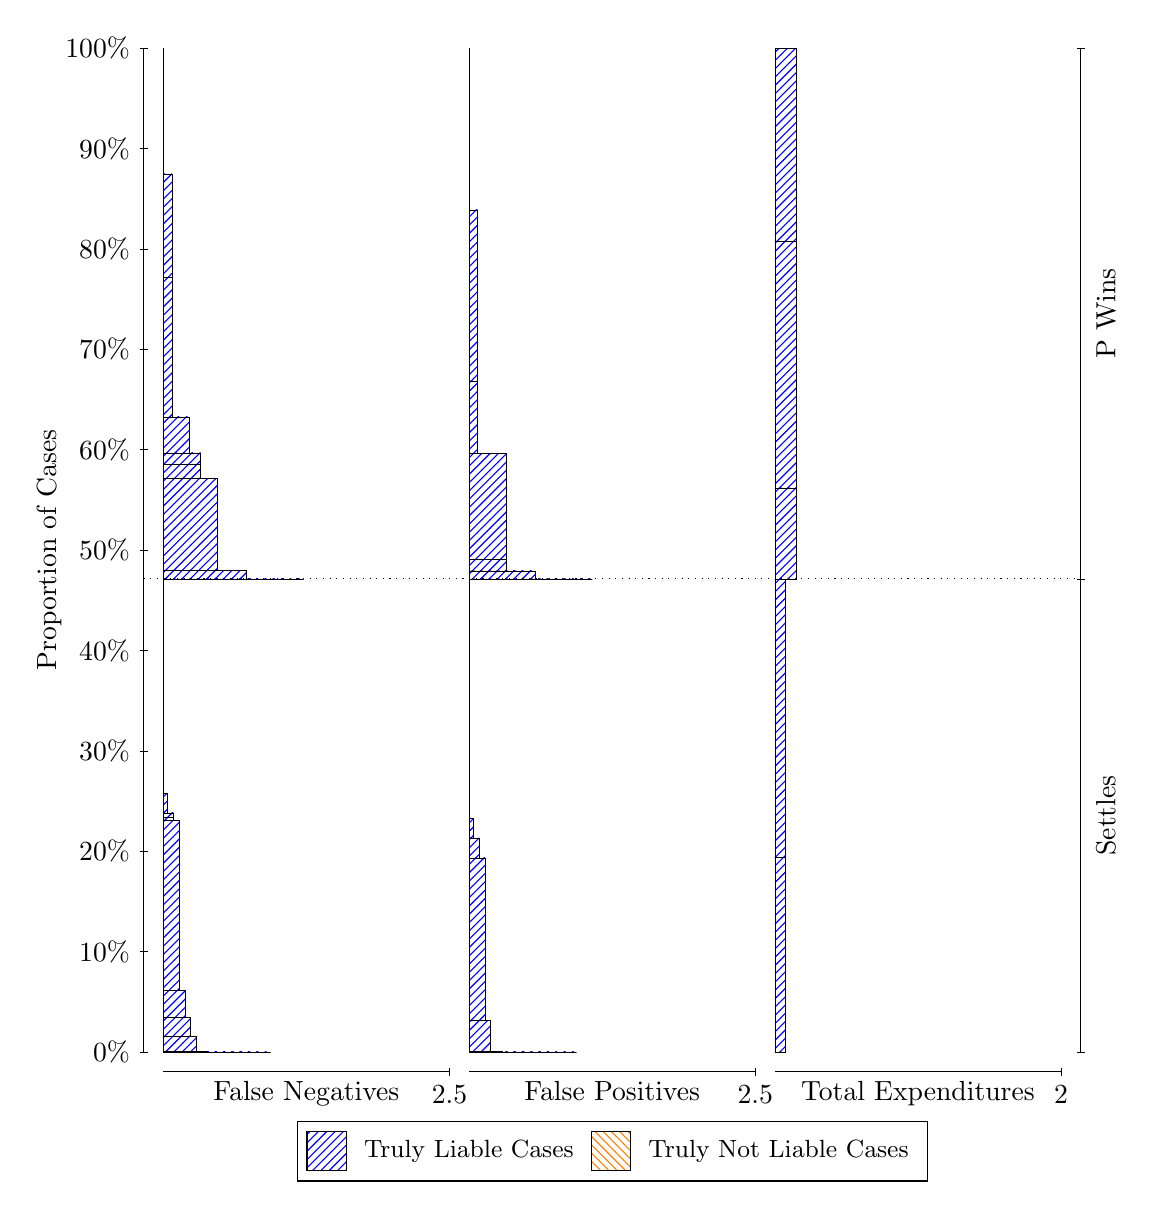
\begin{tikzpicture}
\draw[black, very thin] (1.5,1.75) -- (1.5,14.5);
\node[rotate=90, text=black, anchor=center] at (0.3, 8.125) {Proportion of Cases};
\draw[black, very thin] (1.45,1.75) -- (1.55,1.75);
\node[text=black, anchor=east] at (1.45, 1.75) {0\%};
\draw[black, very thin] (1.45,3.025) -- (1.55,3.025);
\node[text=black, anchor=east] at (1.45, 3.025) {10\%};
\draw[black, very thin] (1.45,4.3) -- (1.55,4.3);
\node[text=black, anchor=east] at (1.45, 4.3) {20\%};
\draw[black, very thin] (1.45,5.575) -- (1.55,5.575);
\node[text=black, anchor=east] at (1.45, 5.575) {30\%};
\draw[black, very thin] (1.45,6.85) -- (1.55,6.85);
\node[text=black, anchor=east] at (1.45, 6.85) {40\%};
\draw[black, very thin] (1.45,8.125) -- (1.55,8.125);
\node[text=black, anchor=east] at (1.45, 8.125) {50\%};
\draw[black, very thin] (1.45,9.4) -- (1.55,9.4);
\node[text=black, anchor=east] at (1.45, 9.4) {60\%};
\draw[black, very thin] (1.45,10.675) -- (1.55,10.675);
\node[text=black, anchor=east] at (1.45, 10.675) {70\%};
\draw[black, very thin] (1.45,11.95) -- (1.55,11.95);
\node[text=black, anchor=east] at (1.45, 11.95) {80\%};
\draw[black, very thin] (1.45,13.225) -- (1.55,13.225);
\node[text=black, anchor=east] at (1.45, 13.225) {90\%};
\draw[black, very thin] (1.45,14.5) -- (1.55,14.5);
\node[text=black, anchor=east] at (1.45, 14.5) {100\%};

\draw[black, very thin] (13.4,1.75) -- (13.4,14.5);
\draw[black, very thin] (13.35,1.75) -- (13.45,1.75);
\node[anchor=west] at (13.35, 1.75) {};
\draw[black, very thin] (13.35,7.7579) -- (13.45,7.7579);
\node[anchor=west] at (13.35, 7.7579) {};
\draw[black, very thin] (13.35,14.5) -- (13.45,14.5);
\node[anchor=west] at (13.35, 14.5) {};

\draw[black, very thin, pattern color=blue, pattern=north east lines] (1.75,1.75) rectangle (3.1125,1.75);
\draw[black, very thin, pattern color=blue, pattern=north east lines] (1.75,1.75) rectangle (2.9672,1.75);
\draw[black, very thin, pattern color=blue, pattern=north east lines] (1.75,1.75) rectangle (2.8218,1.75);
\draw[black, very thin, pattern color=blue, pattern=north east lines] (1.75,1.75) rectangle (2.7492,1.75);
\draw[black, very thin, pattern color=blue, pattern=north east lines] (1.75,1.75) rectangle (2.6765,1.75);
\draw[black, very thin, pattern color=blue, pattern=north east lines] (1.75,1.75) rectangle (2.6038,1.75);
\draw[black, very thin, pattern color=blue, pattern=north east lines] (1.75,1.75) rectangle (2.5312,1.7505);
\draw[black, very thin, pattern color=blue, pattern=north east lines] (1.75,1.7505) rectangle (2.4585,1.751);
\draw[black, very thin, pattern color=blue, pattern=north east lines] (1.75,1.751) rectangle (2.3858,1.7515);
\draw[black, very thin, pattern color=blue, pattern=north east lines] (1.75,1.7515) rectangle (2.3132,1.754);
\draw[black, very thin, pattern color=blue, pattern=north east lines] (1.75,1.754) rectangle (2.2405,1.7583);
\draw[black, very thin, pattern color=blue, pattern=north east lines] (1.75,1.7583) rectangle (2.1678,1.9439);
\draw[black, very thin, pattern color=blue, pattern=north east lines] (1.75,1.9439) rectangle (2.0952,2.1941);
\draw[black, very thin, pattern color=blue, pattern=north east lines] (1.75,2.1941) rectangle (2.0225,2.5325);
\draw[black, very thin, pattern color=blue, pattern=north east lines] (1.75,2.5325) rectangle (1.9498,4.6869);
\draw[black, very thin, pattern color=blue, pattern=north east lines] (1.75,4.6869) rectangle (1.8772,4.7288);
\draw[black, very thin, pattern color=blue, pattern=north east lines] (1.75,4.7288) rectangle (1.8772,4.7864);
\draw[black, very thin, pattern color=blue, pattern=north east lines] (1.75,4.7864) rectangle (1.8045,5.0381);
\draw[black, very thin, pattern color=orange, pattern=north west lines] (1.75,5.0381) rectangle (1.75,5.0381);
\draw[black, very thin, pattern color=blue, pattern=north east lines] (1.75,5.0381) rectangle (1.75,7.7579);
\draw[black, very thin, pattern color=blue, pattern=north east lines] (1.75,7.7579) rectangle (3.5303,7.7579);
\draw[black, very thin, pattern color=blue, pattern=north east lines] (1.75,7.7579) rectangle (3.167,7.759);
\draw[black, very thin, pattern color=blue, pattern=north east lines] (1.75,7.759) rectangle (2.949,7.759);
\draw[black, very thin, pattern color=blue, pattern=north east lines] (1.75,7.759) rectangle (2.8037,7.8616);
\draw[black, very thin, pattern color=blue, pattern=north east lines] (1.75,7.8616) rectangle (2.5857,7.8618);
\draw[black, very thin, pattern color=blue, pattern=north east lines] (1.75,7.8618) rectangle (2.4403,9.0314);
\draw[black, very thin, pattern color=blue, pattern=north east lines] (1.75,9.0314) rectangle (2.2223,9.211);
\draw[black, very thin, pattern color=blue, pattern=north east lines] (1.75,9.211) rectangle (2.2223,9.3586);
\draw[black, very thin, pattern color=blue, pattern=north east lines] (1.75,9.3586) rectangle (2.077,9.8143);
\draw[black, very thin, pattern color=blue, pattern=north east lines] (1.75,9.8143) rectangle (1.859,11.591);
\draw[black, very thin, pattern color=blue, pattern=north east lines] (1.75,11.591) rectangle (1.859,12.902);
\draw[black, very thin, pattern color=orange, pattern=north west lines] (1.75,12.902) rectangle (1.75,12.902);
\draw[black, very thin, pattern color=blue, pattern=north east lines] (1.75,12.902) rectangle (1.75,14.5);
\draw[black, very thin, pattern color=orange, pattern=north west lines] (5.6333,1.75) rectangle (6.9958,1.75);
\draw[black, very thin, pattern color=blue, pattern=north east lines] (5.6333,1.75) rectangle (6.9958,1.75);
\draw[black, very thin, pattern color=orange, pattern=north west lines] (5.6333,1.75) rectangle (6.7052,1.75);
\draw[black, very thin, pattern color=blue, pattern=north east lines] (5.6333,1.75) rectangle (6.7052,1.75);
\draw[black, very thin, pattern color=blue, pattern=north east lines] (5.6333,1.75) rectangle (6.6325,1.75);
\draw[black, very thin, pattern color=orange, pattern=north west lines] (5.6333,1.75) rectangle (6.5598,1.75);
\draw[black, very thin, pattern color=blue, pattern=north east lines] (5.6333,1.75) rectangle (6.5598,1.75);
\draw[black, very thin, pattern color=orange, pattern=north west lines] (5.6333,1.75) rectangle (6.4145,1.75);
\draw[black, very thin, pattern color=blue, pattern=north east lines] (5.6333,1.75) rectangle (6.4145,1.75);
\draw[black, very thin, pattern color=blue, pattern=north east lines] (5.6333,1.75) rectangle (6.3418,1.75);
\draw[black, very thin, pattern color=orange, pattern=north west lines] (5.6333,1.75) rectangle (6.2692,1.75);
\draw[black, very thin, pattern color=blue, pattern=north east lines] (5.6333,1.75) rectangle (6.2692,1.7514);
\draw[black, very thin, pattern color=blue, pattern=north east lines] (5.6333,1.7514) rectangle (6.1965,1.7514);
\draw[black, very thin, pattern color=orange, pattern=north west lines] (5.6333,1.7514) rectangle (6.1238,1.7514);
\draw[black, very thin, pattern color=blue, pattern=north east lines] (5.6333,1.7514) rectangle (6.1238,1.7524);
\draw[black, very thin, pattern color=blue, pattern=north east lines] (5.6333,1.7524) rectangle (6.0512,1.7565);
\draw[black, very thin, pattern color=orange, pattern=north west lines] (5.6333,1.7565) rectangle (5.9785,1.7565);
\draw[black, very thin, pattern color=blue, pattern=north east lines] (5.6333,1.7565) rectangle (5.9785,1.7595);
\draw[black, very thin, pattern color=blue, pattern=north east lines] (5.6333,1.7595) rectangle (5.9785,1.7611);
\draw[black, very thin, pattern color=blue, pattern=north east lines] (5.6333,1.7611) rectangle (5.9058,2.1472);
\draw[black, very thin, pattern color=orange, pattern=north west lines] (5.6333,2.1472) rectangle (5.8332,2.1472);
\draw[black, very thin, pattern color=blue, pattern=north east lines] (5.6333,2.1472) rectangle (5.8332,4.213);
\draw[black, very thin, pattern color=blue, pattern=north east lines] (5.6333,4.213) rectangle (5.8332,4.2135);
\draw[black, very thin, pattern color=blue, pattern=north east lines] (5.6333,4.2135) rectangle (5.7605,4.4698);
\draw[black, very thin, pattern color=blue, pattern=north east lines] (5.6333,4.4698) rectangle (5.6878,4.7214);
\draw[black, very thin, pattern color=blue, pattern=north east lines] (5.6333,4.7214) rectangle (5.6333,7.7579);
\draw[black, very thin, pattern color=orange, pattern=north west lines] (5.6333,7.7579) rectangle (7.1957,7.7579);
\draw[black, very thin, pattern color=blue, pattern=north east lines] (5.6333,7.7579) rectangle (7.1957,7.7579);
\draw[black, very thin, pattern color=orange, pattern=north west lines] (5.6333,7.7579) rectangle (6.8323,7.7579);
\draw[black, very thin, pattern color=blue, pattern=north east lines] (5.6333,7.7579) rectangle (6.8323,7.759);
\draw[black, very thin, pattern color=orange, pattern=north west lines] (5.6333,7.759) rectangle (6.469,7.759);
\draw[black, very thin, pattern color=blue, pattern=north east lines] (5.6333,7.759) rectangle (6.469,7.8596);
\draw[black, very thin, pattern color=orange, pattern=north west lines] (5.6333,7.8596) rectangle (6.251,7.8596);
\draw[black, very thin, pattern color=blue, pattern=north east lines] (5.6333,7.8596) rectangle (6.251,7.8596);
\draw[black, very thin, pattern color=orange, pattern=north west lines] (5.6333,7.8596) rectangle (6.1057,7.8596);
\draw[black, very thin, pattern color=blue, pattern=north east lines] (5.6333,7.8596) rectangle (6.1057,8.0072);
\draw[black, very thin, pattern color=blue, pattern=north east lines] (5.6333,8.0072) rectangle (6.1057,9.3558);
\draw[black, very thin, pattern color=orange, pattern=north west lines] (5.6333,9.3558) rectangle (5.8877,9.3558);
\draw[black, very thin, pattern color=blue, pattern=north east lines] (5.6333,9.3558) rectangle (5.8877,9.3563);
\draw[black, very thin, pattern color=blue, pattern=north east lines] (5.6333,9.3563) rectangle (5.7423,10.272);
\draw[black, very thin, pattern color=blue, pattern=north east lines] (5.6333,10.272) rectangle (5.7423,12.444);
\draw[black, very thin, pattern color=orange, pattern=north west lines] (5.6333,12.444) rectangle (5.6333,12.444);
\draw[black, very thin, pattern color=blue, pattern=north east lines] (5.6333,12.444) rectangle (5.6333,14.5);
\draw[black, very thin, pattern color=orange, pattern=north west lines] (9.5167,1.75) rectangle (9.6529,1.75);
\draw[black, very thin, pattern color=blue, pattern=north east lines] (9.5167,1.75) rectangle (9.6529,4.217);
\draw[black, very thin, pattern color=orange, pattern=north west lines] (9.5167,4.217) rectangle (9.6529,4.217);
\draw[black, very thin, pattern color=blue, pattern=north east lines] (9.5167,4.217) rectangle (9.6529,7.7579);
\draw[black, very thin, pattern color=orange, pattern=north west lines] (9.5167,7.7579) rectangle (9.7892,7.7579);
\draw[black, very thin, pattern color=blue, pattern=north east lines] (9.5167,7.7579) rectangle (9.7892,8.9138);
\draw[black, very thin, pattern color=orange, pattern=north west lines] (9.5167,8.9138) rectangle (9.7892,8.9138);
\draw[black, very thin, pattern color=blue, pattern=north east lines] (9.5167,8.9138) rectangle (9.7892,12.044);
\draw[black, very thin, pattern color=orange, pattern=north west lines] (9.5167,12.044) rectangle (9.7892,12.044);
\draw[black, very thin, pattern color=blue, pattern=north east lines] (9.5167,12.044) rectangle (9.7892,14.5);
\draw[black, dotted] (1.5,7.7579) -- (13.4,7.7579);
\draw[black, very thin] (1.75,1.5) -- (5.3833,1.5);
\node[text=black, anchor=north] at (3.5667, 1.5) {False Negatives};
\draw[black, very thin] (5.3833,1.45) -- (5.3833,1.55);
\node[text=black, anchor=north] at (5.3833, 1.45) {2.5};

\draw[black, very thin] (5.6333,1.5) -- (9.2667,1.5);
\node[text=black, anchor=north] at (7.45, 1.5) {False Positives};
\draw[black, very thin] (9.2667,1.45) -- (9.2667,1.55);
\node[text=black, anchor=north] at (9.2667, 1.45) {2.5};

\draw[black, very thin] (9.5167,1.5) -- (13.15,1.5);
\node[text=black, anchor=north] at (11.333, 1.5) {Total Expenditures};
\draw[black, very thin] (13.15,1.45) -- (13.15,1.55);
\node[text=black, anchor=north] at (13.15, 1.45) {2};

\node[text=black, centered, rotate=90] at (13.72, 4.7539) {Settles};
\node[text=black, centered, rotate=90] at (13.72, 11.129) {P Wins};

\draw (7.449999999999999,1.5) node[draw=none] (baseCoordinate) {};
\begin{scope}[align=center]
        \matrix[scale=0.5, draw=black, below=0.5cm of baseCoordinate, nodes={draw}, column sep=0.1cm]{
            \node[rectangle, draw, minimum width=0.5cm, minimum height=0.5cm, pattern color=blue, pattern=north east lines] {}; &
            \node[draw=none, font=\small, text=black] (B) {Truly Liable Cases}; &
            \node[rectangle, draw, minimum width=0.5cm, minimum height=0.5cm, pattern color=orange, pattern=north west lines] {}; &
            \node[draw=none, font=\small, text=black] (B) {Truly Not Liable Cases}; \\
            };
\end{scope}

\end{tikzpicture}
\end{document}